\documentclass{article}
\usepackage{tikz}
\usepackage{circuitikz}
\usepackage{pst-circ}
\usepackage{amsmath}

\usetikzlibrary{circuits.logic.US}
%\usepackage[siunitx]{circuitikz}%



\linespread{1.6}

\begin{document}




\begin{tikzpicture}
\draw (0,0) -- (4,0) -- (4,4) -- (0,4) -- (0,0);
\end{tikzpicture}



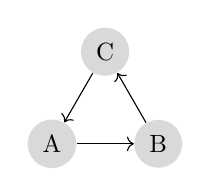
\begin{tikzpicture}[scale=.9, transform shape]
\tikzstyle{every node} = [circle, fill=gray!30]
\node (a) at (0, 0) {A};
\node (b) at +(0: 1.5) {B};
\node (c) at +(60: 1.5) {C};
\foreach \from/\to in {a/b, b/c, c/a}
\draw [->] (\from) -- (\to);
\end{tikzpicture}


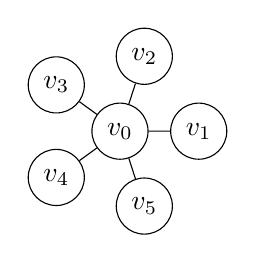
\begin{tikzpicture}
\tikzstyle{every node}=[draw,shape=circle];
\node (v0) at (0:0) {$v_0$};
\node (v1) at ( 0:1) {$v_1$};
\node (v2) at ( 72:1) {$v_2$};
\node (v3) at (2*72:1) {$v_3$};
\node (v4) at (3*72:1) {$v_4$};
\node (v5) at (4*72:1) {$v_5$};
\draw (v0) -- (v1)
(v0) -- (v2)
(v0) -- (v3)
(v0) -- (v4)
(v0) -- (v5);
\end{tikzpicture}

\begin{tikzpicture}
\draw(0,0) parabola (4,4);
\end{tikzpicture}

\begin{tikzpicture}
\draw(2,2) circle (3cm);
\end{tikzpicture}

\begin{tikzpicture}
\draw[red,thick,dashed](2,2) circle (3cm);
\end{tikzpicture}


\begin{tikzpicture}
\draw[step=1cm,gray,very thin](-2,-2) grid (6,6);
\end{tikzpicture}

\newpage

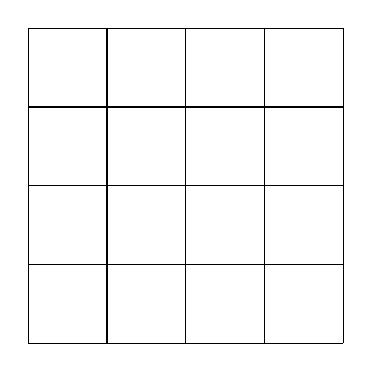
\begin{tikzpicture}
\draw[step=1cm,black,thin](-2,-2) grid (2,2);
\end{tikzpicture}

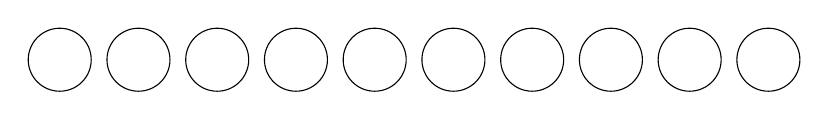
\begin{tikzpicture}
\foreach \x in {0,...,9}
\draw (\x,0) circle (0.4);
\end{tikzpicture}


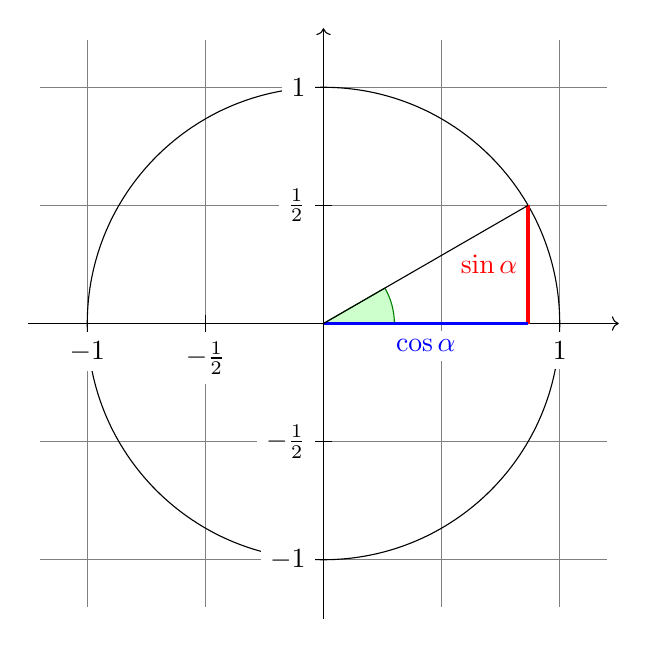
\begin{tikzpicture}[scale=3]
\draw[step=.5cm, gray, very thin] (-1.2,-1.2)
grid (1.2,1.2);
\filldraw[fill=green!20,draw=green!50!black]
(0,0) -- (3mm,0mm) arc (0:30:3mm) -- cycle;
\draw[->] (-1.25,0) -- (1.25,0) coordinate (x
axis);
\draw[->] (0,-1.25) -- (0,1.25) coordinate (y
axis);
\draw (0,0) circle (1cm);
\draw[very thick,red] (30:1cm) --node[left,fill=white] {$\sin \alpha$} (30:1cm |- x
axis);
\draw[very thick,blue] (30:1cm |- x axis) --node[below=2pt,fill=white] {$\cos \alpha$} (0,0);
\draw (0,0) -- (30:1cm);
\foreach \x/\xtext in {-1, -0.5/-\frac{1}{2}, 1}
\draw (\x cm,1pt) -- (\x cm,-1pt)
node[anchor=north,fill=white] {$\xtext$};
\foreach \y/\ytext in {-1, -0.5/-\frac{1}{2},
0.5/\frac{1}{2}, 1}
\draw (1pt,\y cm) -- (-1pt,\y cm)
node[anchor=east,fill=white] {$\ytext$};
\end{tikzpicture}


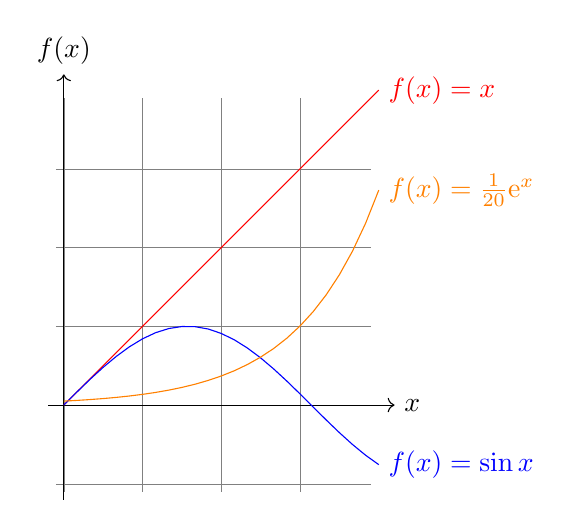
\begin{tikzpicture}[domain=0:4]
\draw[very thin,color=gray] (-0.1,-1.1) grid
(3.9,3.9);
\draw[->] (-0.2,0) -- (4.2,0) node[right] {$x$};
\draw[->] (0,-1.2) -- (0,4.2) node[above] {$f(x)$};
\draw[color=red]    plot (\x,\x)            
node[right] {$f(x) =x$};
\draw[color=blue]   plot (\x,{sin(\x r)})   
node[right] {$f(x) = \sin x$};
\draw[color=orange] plot (\x,{0.05*exp(\x)})
node[right] {$f(x) = \frac{1}{20} \mathrm e^x$};
\end{tikzpicture}



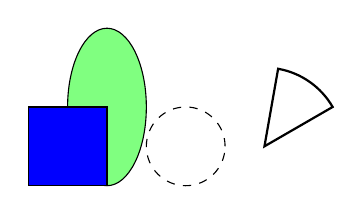
\begin{tikzpicture}
\draw[style=dashed] (2,.5) circle (0.5);
\draw[fill=green!50] (1,1)
ellipse (.5 and 1);
\draw[fill=blue] (0,0) rectangle (1,1);
\draw[style=thick]
(3,.5) -- +(30:1) arc(30:80:1) -- cycle;
\end{tikzpicture}



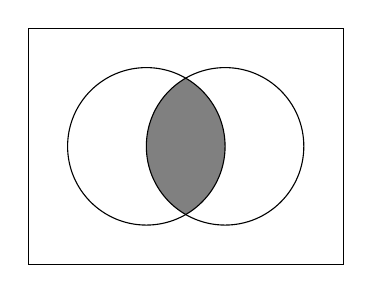
\begin{tikzpicture}
\draw (-2, 1.5) rectangle (2, -1.5);
\begin{scope}
\clip (-0.5, 0) circle (1);
\clip ( 0.5, 0) circle (1);
\fill[color=gray] (-2,1.5)
rectangle (2,-1.5);
\end{scope}
\draw (-0.5, 0) circle (1);
\draw ( 0.5, 0) circle (1);
\end{tikzpicture}


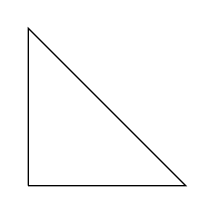
\begin{tikzpicture}
\draw (0,0) -- (0,2) -- (2,0)-- (0,0);
\end{tikzpicture}


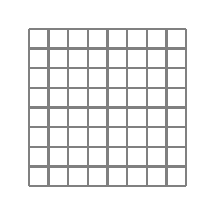
\begin{tikzpicture}
\draw[step=.25cm,gray,thick]
(-1,-1) grid (1,1);
\end{tikzpicture}


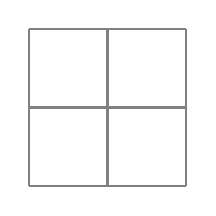
\begin{tikzpicture}
\draw[step=1cm,gray,thick]
(-1,-1) grid (1,1);
\end{tikzpicture}


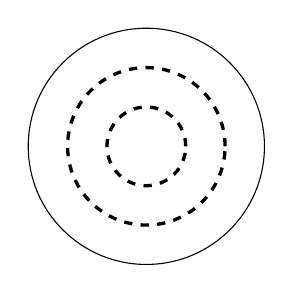
\begin{tikzpicture}
\begin{scope}[very thick,dashed]
\draw (0,0) circle (.5cm);
\draw (0,0) circle (1cm);
\end{scope}
\draw[thin] (0,0) circle (1.5cm);
\end{tikzpicture}



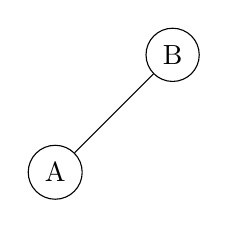
\begin{tikzpicture}
\draw (1,1) node[anchor=north east,circle,
draw]{A} -- (2,2) node[anchor=south west,
circle,draw]{B};
\end{tikzpicture}



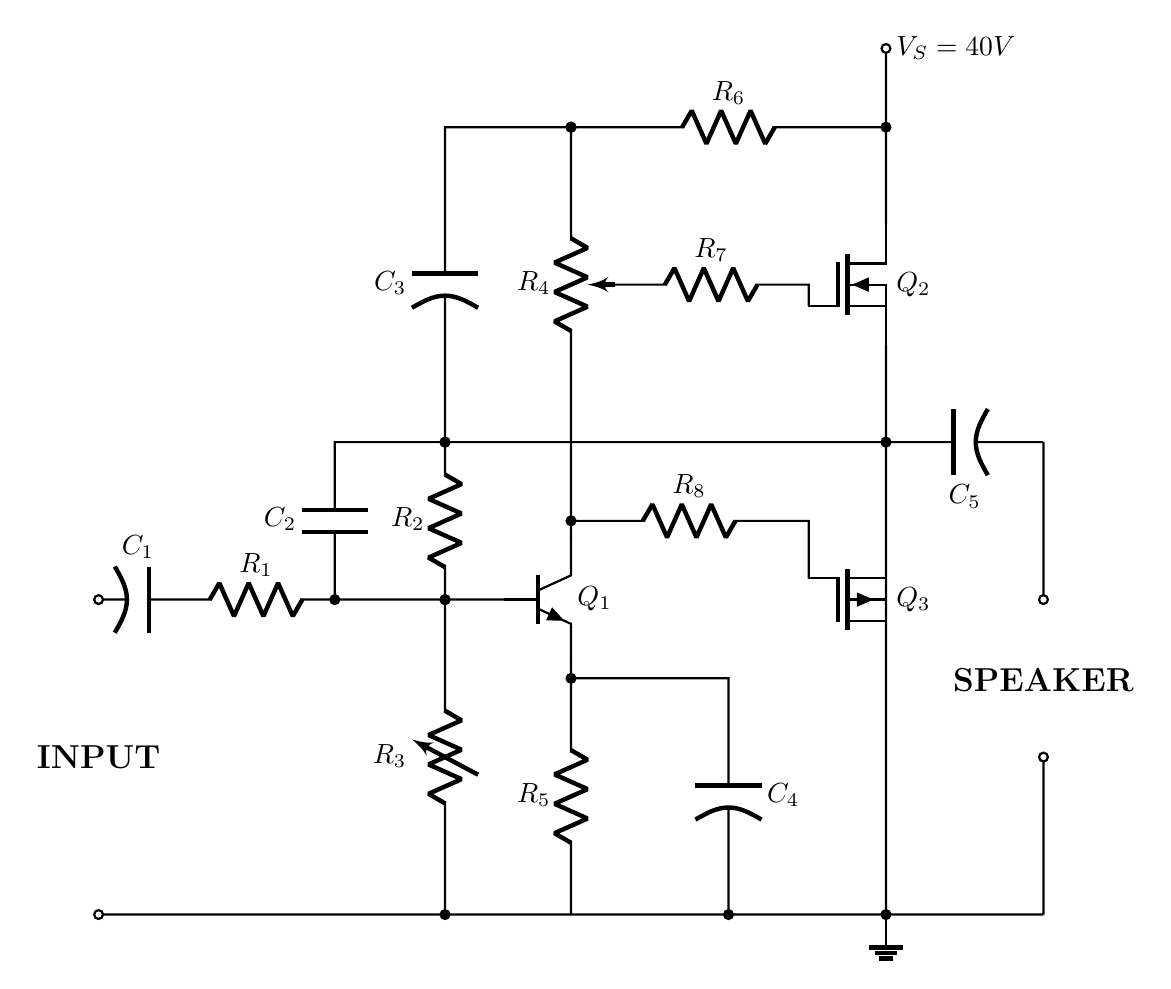
\begin{tikzpicture}[scale=2]
  \draw[color=black, thick]
    (0,0) to [short,o-] (6,0){} % Baseline for connection to ground
    % Input and ground
    (0,1) node[]{\large{\textbf{INPUT}}}
    % Connection of passive components
    (5,0) node[ground]{} node[circ](4.5,0){}
    (0,2) to [pC, l=$C_1$, o-] (0.5,2)
    to [R,l=$R_1$,](1.5,2)
    to node[short]{}(2.6,2)
    (1.5,2) to [C, l=$C_2$, *-] (1.5,3) -| (5,3)
    (2.2,2) to [R, l=$R_2$, *-*] (2.2,3)
    (2.2,3) to [pC, l=$C_3$, *-] (2.2,5) -| (3,5)
    % Transistor Bipolar Q1
    (3,0) to [R,l=$R_5$,-*] (3,1.5)
    to [Tnpn,n=npn1] (3,2.5)
    (npn1.E) node[right=3mm, above=5mm]{$Q_1$} % Labelling the NPN transistor
    (4,0) to [pC, l_=$C_4$, *-] (4, 1.5)--(3,1.5)
    (2.2,0) to [vR, l=$R_3$, *-*] (2.2,2)
    (3,2.5) to node[short]{}(3,3)
    (3,5) to [pR, n=pot1, l_=$R_4$, *-] (3,3)
    (3,5) to [R, l=$R_6$, *-] (5,5)
    to [short,*-o](5,5.5) node[right]{$V_S=40 V$}
    % Mosfet Transistors
    (5,3) to [Tnigfetd,n=mos1] (5,5)
    (mos1.B) node[anchor=west]{$Q_2$} % Labelling MOSFET Q2 Transistor
    (pot1.wiper)  to [R, l=$R_7$] (4.5,4) -| (mos1.G)
    (5,1.5) to [Tpigfetd,n=mos2] (5,2.5)
    (5,0) to (mos2.S)
    (3,2.5) to [R, l=$R_8$, *-] (4.5,2.5)
    -| (mos2.G)
    (mos2.B) node[anchor=west]{$Q_3$} % Labelling MOSFET Q3 Transistor
    % Output
    (6,3) to [pC, l=$C_5$,-*](5,3)
    (6,3) to [short,-o] (6,2){}
    (mos1.S)--(mos2.D)
    (6,0) to [short,-o] (6,1){} node[above=7mm]{\large{\textbf{SPEAKER}}}
    ;
\end{tikzpicture}

\newpage



\begin{circuitikz} \draw
(0,2) node[and port] (myand1) {}
(0,0) node[and port] (myand2) {}
(2,1) node[xnor port] (myxnor) {};
(myand1.out) | (myxnor.in 1)
(myand2.out) | (myxnor.in 2)
\end{circuitikz}


\begin{circuitikz} \draw
(0,2) node[and port] (myand1) {}
(0,0) node[and port] (myand2) {}
(2,1) node[xnor port] (myxnor) {}
(myand1.out) -- (myxnor.in 1)
(myand2.out) -- (myxnor.in 2);
\end{circuitikz}

\tikzstyle{branch}=[fill,shape=circle,minimum size=3pt,inner sep=0pt]
\begin{tikzpicture}[label distance=2mm]

    \node (x3) at (0,0) {$x_3$};
    \node (x2) at (1,0) {$x_2$};
    \node (x1) at (2,0) {$x_1$};
    \node (x0) at (3,0) {$x_0$};

    \node[not gate US, draw, rotate=-90] at ($(x2)+(0.5,-1)$) (Not2) {};
    \node[not gate US, draw, rotate=-90] at ($(x1)+(0.5,-1)$) (Not1) {};
    \node[not gate US, draw, rotate=-90] at ($(x0)+(0.5,-1)$) (Not0) {};

    \node[or gate US, draw, logic gate inputs=nnn] at ($(x0)+(2,-2)$) (Or1) {};
    \node[or gate US, draw, logic gate inputs=nnnn] at ($(Or1)+(0,-1)$) (Or2) {};
    \node[or gate US, draw, logic gate inputs=nnn] at ($(Or2)+(0,-1)$) (Or3) {};
    \node[xor gate US, draw, logic gate inputs=nn] at ($(Or3)+(0,-1)$) (Xor1) {};
    \node[and gate US, draw, logic gate inputs=nn, anchor=input 1] at ($(Or3.output)+(1,0)$) (And1) {};
    \node[nor gate US, draw, logic gate inputs=nn, anchor=input 1] at ($(Or2.output -| And1.output)+(1,0)$) (Nor1) {};
    \node[and gate US, draw, logic gate inputs=nn, anchor=input 1] at ($(Or1.output -| Nor1.output)+(1,0)$) (And2) {};

    \foreach \i in {2,1,0}
    {
        \path (x\i) -- coordinate (punt\i) (x\i |- Not\i.input);
        \draw (punt\i) node[branch] {} -| (Not\i.input);
    }
    \draw (x3) |- (Or2.input 1);
    \draw (x3 |- Or1.input 1) node[branch] {} -- (Or1.input 1);
    \draw (x2) |- (Xor1.input 1);
    \draw (x2 |- Or3.input 1) node[branch] {} -- (Or3.input 1);
    \draw (Not2.output) |- (Or2.input 2);
    \draw (x1) |- (Or3.input 2);
    \draw (x1 |- Or1.input 2) node[branch] {} -- (Or1.input 2);
    \draw (Not1.output) |- (Xor1.input 2);
    \draw (Not1.output |- Or2.input 3) node[branch] {} -- (Or2.input 3);
    \draw (x0) |- (Or2.input 4);
    \draw (Not0.output) |- (Or3.input 3);
    \draw (Not0.output |- Or1.input 3) node[branch] {} -- (Or1.input 3);
    \draw (Or3.output) -- (And1.input 1);
    \draw (Xor1.output) -- ([xshift=0.5cm]Xor1.output) |- (And1.input 2);
    \draw (Or2.output) -- (Nor1.input 1);
    \draw (And1.output) -- ([xshift=0.5cm]And1.output) |- (Nor1.input 2);
    \draw (Or1.output) -- (And2.input 1);
    \draw (Nor1.output) -- ([xshift=0.5cm]Nor1.output) |- (And2.input 2);
    \draw (And2.output) -- ([xshift=0.5cm]And2.output) node[above] {$f_1$};

\end{tikzpicture}




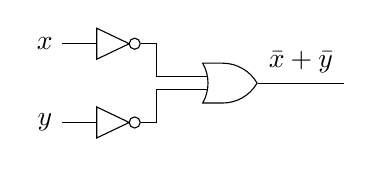
\begin{tikzpicture}
    \node (x) at (0, 1) {$x$};
    \node (y) at (0, 0) {$y$};

    \node[not gate US, draw] at ($(x) + (0.8, 0)$) (notx) {};
    \node[not gate US, draw] at ($(y) + (0.8, 0)$) (noty) {};
    \node[or gate US, draw, rotate=0, logic gate inputs=nn] at ($(noty) + (1.5, 0.5)$) (xory) {};

    \draw (x) -- (notx.input);
    \draw (y) -- (noty.input);

    \draw (notx.output) -- ([xshift=0.2cm]notx.output) |- (xory.input 1);
    \draw (noty.output) -- ([xshift=0.2cm]noty.output) |- (xory.input 2);

    \draw (xory.output) -- node[above]{$\bar x + \bar y$} ($(xory) + (1.5, 0)$);
\end{tikzpicture}




\begin{tikzpicture}
    \node (x) at (0, 2) {$x$};
    \node (y) at (0, 1) {$y$};
    \node (z) at (0, 0) {$z$};

    \node[not gate US, draw] at ($(x) + (0.8, 0)$) (notx) {};
    \node[not gate US, draw] at ($(y) + (0.8, 0)$) (noty) {};
    \node[nor gate US, draw, rotate=0, logic gate inputs=nnnn] at ($(noty) + (2, 0.085)$) (xory) {};

    \draw (x) -- (notx.input);
    \draw (y) -- (noty.input);

    \path ($(notx.input) + (0.2, 0)$) -- coordinate (puntx) (x |- notx);
    \draw (x) -- (puntx) node[branch] {} |- ($(notx.output) + (0.4, 0.4)$) |- (xory.input 1);

    \draw (notx.output) -- ([xshift=0.2cm]notx.output) |- (xory.input 2);
    \draw (noty.output) -- ([xshift=0.2cm]noty.output) |- (xory.input 3);
    \draw (z) -| ($(noty.output) + (0.2, -0.5)$) |- (xory.input 4);

    \draw (xory.output) -- node[above]{$\overline{x + \bar x + \bar y + z}$} ($(xory) + (3, 0)$);
\end{tikzpicture}


\newpage


\begin{tikzpicture}
    % axes
    \draw[->](-3.5, 0) -- (4.2, 0) node[right] {$x$};
    \draw[->](0, -pi) -- (0, 4.2) node[above] {$y$};

    % graphs
    \draw[scale=0.5, domain=-3:3, smooth, variable=\x, blue]
        plot ({\x}, {\x*\x});
    \draw[domain=-pi:pi, smooth, variable=\x, red]
        plot ({\x}, {sin(deg(\x))});
\end{tikzpicture}





\begin{tikzpicture}[x=1cm, y=1cm, z=-0.6cm]
    % Axes
    \draw [->] (0,0,0) -- (4,0,0) node [right] {$x$};
    \draw [->] (0,0,0) -- (0,4,0) node [left] {$y$};
    \draw [->] (0,0,0) -- (0,0,4) node [left] {$z$};
    % Vectors
    \draw [->, thick] (0,0,0) -- (2,2,0);
    \draw [->, thick] (0,0,0) -- (2,0,1);
    % Ticks
        \foreach \i in {1,2}
    {
    \draw (-0.1,\i,0) -- ++ (0.2,0,0);
    \draw (\i,-0.1,0) -- ++ (0,0.2,0);
    \draw (-0.1,0,\i) -- ++ (0.2,0,0);
    }
    % Dashed lines
    \draw [loosely dashed]
        (0,2,0) -- (2,2,0) -- (2,0,0)
        (0,0,1) -- (2,0,1) -- (2,0,0)
        ;
    % Labels
     \node [right] at (2,2,0) {$\begin{bmatrix}
                                2\\2\\0
                               \end{bmatrix}$};
   \node [below] at (2,0,1) {$\begin{bmatrix}
                               2\\0\\1
                              \end{bmatrix}$};

\end{tikzpicture}














\end{document}